\scanpage{401}
\mspage{203}

\unsure{arithmetizations|arithmetization} of $\pi'_i$ --- which
would amount to the bijectivity of
\[
\widehat{\widehat{\mathcal T}}/\mathcal N_a
\longrightarrow
\widehat{\widehat{\mathcal G}}'/\unsure{M_{a'}^{\natural}|M_{a'}^{\sharp}}
\simeq \widehat{\widehat{\mathcal T}}'/\mathcal N_{a'},
\]
which \inserted{would} hardly have any reason to be except if
one admitted
$\widehat{\widehat{\mathcal T}}(\pi)\xrightarrow{\sim}\unsure{\widehat{\widehat{\mathcal G}}|\widehat{\mathcal G}}(\pi'_i)$,
which seems quite problematic to me.

\margin{\figure{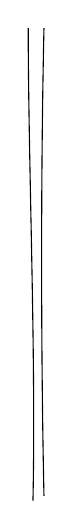
\begin{tikzpicture}[x=1cm,y=1cm,baseline=(current bounding box.north)]
\draw[line width=0.4pt] (0,0) .. controls (0.04,1.85) and (-0.06,4.30) .. (-0.06,6.00);
\draw[line width=0.4pt] (0.14,0.06) .. controls (0.10,1.90) and (0.10,4.25) .. (0.14,6.00);
\end{tikzpicture}}}
However, one finds, by the
``plugging the holes'' functor, an equivalence
between the category of \deleted{\unsure{algebraic curves}}
\uuline{outer} \uline{arithmetized} profinite groups with loops,
\inserted{of type $(g,\nu)$,}
and of \uline{arithmetized} profinite groups with loops
(not outer!), of type
$(g,\nu-1)$.

One can propose to try to
specify \deleted{\unsure{by}} the type of properties
which will characterize $\mathcal N_{g,\nu}$ in $\mathcal N'_{g,\nu}=$
$\operatorname{Norm}_{\widehat{\widehat{\mathcal T}}_{g,\nu}}
(\widehat{\mathcal T}_{g,\nu}^{+})$,
\deleted{I \unsure{think} that it}
\inserted{\deleted{\unsure{We shall have}}or again}
$\mathbb{\Gamma}_{g,\nu}$
\deleted{\unsure{for} \illegible{1} $\Gamma'$}
in $\mathbb{\Gamma}'_{g,\nu}=\mathcal N'_{g,\nu}/\widehat{\mathcal T}_{g,\nu}^{+}$.
We have natural homomorphisms

\margin{400}

\scanpage{402}

\[
\tag{15}
\left|
\begin{aligned}
\mathbb{\Gamma}'_{g,\nu}&\longrightarrow\operatorname{Autext}(\widehat{\mathcal T}_{g,\nu}^{+})\\
\mathbb{\Gamma}'_{g,\nu}&\longrightarrow\operatorname{Aut\,ext}(\widehat{\mathcal T}_{g,\nu}^{+!})
\end{aligned}
\right.
\]
and I presume that \deleted{it is a matter} $\mathbb{\Gamma}_{g,\nu}$ will
be describable as the inverse image of a
suitable closed subgroup of one
or the other of the right-hand sides, i.e. that one
can describe it in terms \unsure{of the|of} properties
of outer operations on $\widehat{\mathcal T}_{g,\nu}^{+}$ or
on $\widehat{\mathcal T}_{g,\nu}$. The conditions \textcircled{e} in any
case are indeed of this type (\unsure{property|properties}
of normalizing \unsure{invariant|inscribed} \unsure{subgroups}
\deleted{$\unsure{\mathcal T'_i}$} $\pi'_i$ of $\mathcal T_{g,\nu}^{+!}$ ...).
Of course, one
could impose conditions on outer
\unsure{automorphisms} (of $\widehat{\mathcal T}'{}_{g,\nu}^{+!}$, say),
which are stable under \inserted{successive} passage to
$\widehat{\mathcal T}'{}_{g,\nu-1}^{+!}$, $\widehat{\mathcal T}'{}_{g,\unsure{\nu-2}}^{+!}$ etc ... and
\deleted{for which}\inserted{which are}
generated by the conditions \textcircled{e}. But
it is not at all certain that this

\margin{401}

\scanpage{403}
\mspage{204}

\unsure{will suffice|suffices} to describe the \deleted{$\unsure{\mathcal N_{g,\nu}}$}
$\mathbb{\Gamma}_{g,\nu}\subset\Gamma'_{g,\nu}$,
if only because the condition
becomes vacuous for \deleted{$\unsure{\nu=0}$} the limiting case $\nu=0$
(if $g\geq2$; or for the cases $g=1$, $\nu=1$, or $g=0$, $\nu=3$).

It is possible that one will have to
bring in properties of the $\pi_1$ of
the $\unsure{M_{g,\nu\,\overline{\mathbb Q}_a}}$, linked to the compactification.
It is practically only in the case of
$(g,\nu)=(0,3)$ that one should not expect
conditions of this kind at all.

Let us call ``\unsure{potential algebraic curve|potential algebraic curves}''
(understood, over an unspecified algebraic closure of $\mathbb Q$,)
the datum of \unsure{a|a} \inserted{profinite outer \unsure{group}}
$\pi$ with \unsure{loops|loop} \deleted{profinite}\inserted{\deleted{outer}}
of type $(g,\nu)$, equipped with an arithmetization
$a$, and with a germ of
``admissible'' liftings
\margin{\deleted{\illegible{1}}}
\[
\tag{16}
\mathbb{\Gamma}_{\unsure{a|\bullet}}^{\natural}
\longrightarrow\mathcal N_a.
\]
They form a category (for
isomorphisms, for the moment) If one gives oneself
a torsor $P$ under $\mathbb{\Gamma}_{g,\nu}$
(which \inserted{\unsure{trivially|morally}} amounts to giving oneself an algebraic

\margin{402}

\scanpage{404}
closure $\overline{\mathbb Q}$ of $\mathbb Q$ \ldots) the potential curves
of type $(g,\nu)$ \uline{\unsure{relative|relative}} to this torsor
(\unsure{morally|morally}, \unsure{corresponding|correspond} to algebraic
curves over $\overline{\mathbb Q}$ \ldots) are \inserted{those} equipped in
addition with an \unsure{isomorphism} (``inner'')
\[
(17)\qquad \mathbb P_a\xrightarrow{\sim}P
\]
(defining an isomorphism
\[
(18)\qquad \mathbb{\Gamma}_a\longrightarrow\Gamma_P
 =\operatorname{Aut}_{\mathbb{\Gamma}_{g,\nu}}(P).
\]
\margin{The case where $P$ is the
trivial torsor, is that of the \deleted{\unsure{curves}} outer $\pi$ \unsure{(?)|(18)}
equipped with an oriented \uline{prediscretification} $\alpha$
(whence an \deleted{\illegible{1}} exact \unsure{sequence}
$1\longrightarrow\widehat{\mathcal T}_\alpha\longrightarrow
\mathcal N_\alpha\longrightarrow\mathbb{\Gamma}_\alpha\longrightarrow1$)}

This time, one expects to find
\uline{finite} \unsure{sets} of isomorphisms, instead of
torsors under considerable profinite
groups.

We consider the \deleted{\unsure{P}} \uline{Points} of $\pi$,
as the \inserted{$\pi$-}conjugacy classes
of ``admissible'' \unsure{liftings} of (16),
\unsure{into|or}
\[
(19)\qquad\mathbb{\Gamma}_{\unsure{a|\bullet}}^{\natural}\longrightarrow
\mathcal M_a\subset\widehat{\widehat{\mathcal T}}(\pi)
\]
i.e. a germ of genuine action of $\mathbb{\Gamma}_{\bullet}$
on $\pi$, with
\margin{(20)}
\figure{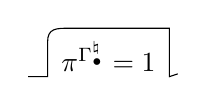
\begin{tikzpicture}[baseline=(eq.base)]
\node[inner sep=0pt,outer sep=0pt] (eq) {$\pi^{\mathbb{\Gamma}_{\bullet}^{\natural}}=1$};
\draw[line width=0.4pt]
([xshift=-12pt,yshift=-2pt]eq.south west)
-- ([xshift=-5pt,yshift=-2pt]eq.south west)
-- ([xshift=-5pt]eq.north west)
.. controls ([xshift=-5pt,yshift=5pt]eq.north west) and ([xshift=-2pt,yshift=5pt]eq.north west) .. ([xshift=3pt,yshift=5pt]eq.north west)
-- ([xshift=5pt,yshift=5pt]eq.north east)
-- ([xshift=5pt,yshift=-2pt]eq.south east)
-- ([xshift=8pt,yshift=-1pt]eq.south east);
\end{tikzpicture}}
(this for \deleted{\unsure{the ad}}
\margin{403}

\scanpage{405}
\mspage{205}
admissibility.

\uline{Preliminary question} Knowledge of
$\pi$, of $\underbrace{\widehat{\mathcal T}_a^+}_{\Sigma_a}
\subset\widehat{\widehat{\mathcal T}}(\pi)$, and \unsure{of a} subgroup
$\Gamma'\subset\widehat{\widehat{\mathcal T}}(\pi)$
(normalizing $\Sigma_a$, \inserted{such that
$\Gamma'\cap\unsure{\Sigma_a|\Sigma_{\bullet}}=(1)$})
\unsure{would it make it possible} to recover the \unsure{arithmetization|arithmetization} of $\pi$
--- and, to begin with, to recover
$\mathcal N_a$ (in which $\Gamma'\cdot\Sigma$ is of finite
index)? \deleted{Is} It \unsure{would suffice|will suffice}, to be able to
answer in the affirmative, to know
that every outer \unsure{isomorphism} $\pi\longrightarrow\pi_{g,\nu}$,
which sends \inserted{$\Sigma$ onto $\widehat{\mathcal T}_{g,\nu}=\Sigma_{g,\nu}$, and}
\unsure{every|the} subgroup of finite
index $\Gamma'\cdot\Sigma$ in $\mathcal N_a$ into $\mathcal N_{g,\nu}$,
is compatible with the \unsure{arithmetizations|arithmetizations}.
Now this amounts \unsure{exactly|exactly} to:

\textcircled{g} (optional, all the same!)
\deleted{every} For every open
subgroup $\mathcal N'$ of $\mathcal N_{g,\nu}$,
the elements of $\widehat{\widehat{\mathcal T}}_{g,\nu}$
\inserted{normalizing $\widehat{\mathcal T}_{g,\nu}$ and}
which carry
$\mathcal N'$ into $\mathcal N_{g,\nu}$, \unsure{are} in $\mathcal N_{g,\nu}$
(\unsure{a fortiori},
$\mathcal N_{g,\nu}$ would be its own normalizer
in $\operatorname{Norm}_{\widehat{\widehat{\mathcal T}}_{g,\nu}}
(\widehat{\mathcal T}_{g,\nu})$.
\margin{404}

\scanpage{406}
With the ``points of $U$'' (defined as conjugacy \unsure{classes}
of ``admissible'' \unsure{liftings} (19)
i.e. satisfying (20), one
makes a groupoid, having
$\pi$ as its outer fundamental group, and on
which $\Gamma^{\unsure{\natural|\sharp}}\subset\mathcal N_a$ operates strictly
(\uline{N.B.} to take a rest, one now gives oneself
$\unsure{\Gamma^{\natural}|\Gamma}$ itself, not \unsure{only|only} a
germ --- \unsure{morally|morally}, this means
that one has a curve defined over a
finite subextension $K$ of $\overline{\mathbb Q}/\mathbb Q$ \ldots\unsure{\}|)}.
The fixed points of $\Gamma$ correspond
to the rational points/$K$, the fixed points under a
closed subgroup $\Gamma'$ to the points rational
over the subextension $K'$ of $\overline{\mathbb Q}/\mathbb Q$ associated
with $\Gamma'$ \ldots)
\margin{405}

\scanpage{407}
\mspage{206}

Now let
\figure{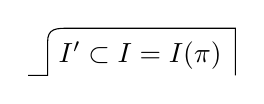
\begin{tikzpicture}[baseline=(eq.base)]
\node[inner sep=0pt,outer sep=0pt] (eq) {$I'\subset I=I(\pi)$};
\draw[line width=0.4pt]
([xshift=-11pt,yshift=-2pt]eq.south west)
-- ([xshift=-4pt,yshift=-2pt]eq.south west)
-- ([xshift=-4pt]eq.north west)
.. controls ([xshift=-4pt,yshift=5pt]eq.north west) and ([xshift=-1pt,yshift=5pt]eq.north west) .. ([xshift=4pt,yshift=5pt]eq.north west)
-- ([xshift=5pt,yshift=5pt]eq.north east)
-- ([xshift=5pt,yshift=-2pt]eq.south east);
\end{tikzpicture}}
be a
subset of $I$, stable under $\Gamma$. One finds
by ``plugging the holes at $I'$'' an
outer group with loops $\pi'$, \deleted{which} and an
outer homomorphism
\[
(20)\qquad \pi^{\unsure{\natural|\sharp}}\longrightarrow\pi'
\]
Besides, $\pi'$ inherits an arithmetization \inserted{$a'$}
from $\pi$ -- and we shall have
\[
(21)\qquad
\left\{
\begin{array}{ccc}
\mathbb{\Gamma}_a & \overset{\sim}{\longrightarrow} & \mathbb{\Gamma}_{a'} \\
\mathbb P_a & \overset{\sim}{\longrightarrow} & \mathbb P_{a'} \\
\unsure{\wr} & & \\
P & &
\end{array}
\right.
\quad\unsure{\leadsto}
\]
so $\pi'$ is defined over \unsure{the|the} same $P$ as
$\mathbb{\Gamma}_a$
(i.e. by making holes in $U$ to
find $U'$, we have not disturbed the
algebraically \unsure{closed|absolute} base field $\overline{\mathbb Q}\ldots$). Besides
we shall have a canonical homomorphism
\[
\widehat{\mathcal T}(\pi)\longrightarrow
\widehat{\mathcal T}(\pi')
\]
inducing
\[
(22)\qquad
\]
\diagram{\begin{tikzcd}[ampersand replacement=\&,column sep=3.2em,row sep=1.8em]
\mathcal N_a \arrow[r] \arrow[d,phantom,"\cup" description] \& \mathcal N_{a'} \arrow[d,phantom,"\cup" description] \\
\widehat{\mathcal T}_a \arrow[r,dash] \& \widehat{\mathcal T}_{a'}
\end{tikzcd}}

\margin{406}

\scanpage{408}

(inducing precisely $\mathbb{\Gamma}_a\longrightarrow\mathbb{\Gamma}_{a'}$ on passing
to the quotients), and one finds, on
composing
\[
\Gamma\;\unsure{\subset|\hookrightarrow}\;\mathcal N_a\longrightarrow\mathcal N_{a'}
\]
a homomorphism which is \unsure{also|also} injective
\[
(23)\qquad\Gamma\hookrightarrow\mathcal N_{a'}
\]
which is a \unsure{quasi-section|quasi section} of $\mathcal N_{a'}$ over $\mathbb{\Gamma}_{a'}$,
So \deleted{\unsure{that|by}}\inserted{under} the proviso of admissibility,
one finds on \deleted{\illegible{1}} $\unsure{\pi'|\pi}$ a structure
of potential algebraic curve, relative
to the same $P$.

\deleted{Admissibility is expressed
\unsure{perhaps by} the condition
\[
(24)\qquad {\pi'}^{\Gamma}=(1)
\]
-- and if need be, we shall put these
conditions (for \unsure{every|$\forall$} $I'\subset I$) into
the definition of the admissibility of}

\deleted{\illegible{1} \unsure{I}} I am really feeling
cramped, for lack of a
definition in due form of ``admissible'' --

\margin{407}

\scanpage{409}
\mspage{207}

I am going to come back to this very soon --- but
for the moment, I feel like noting that,
\deleted{from the fact that $\Gamma$ \unsure{operated} \unsure{trivially}}
\inserted{if $I'\neq\varnothing$,}
the outer group $\pi'$ can be described by
a \inserted{genuine} groupoid, having $I'$ as its set
of objects, and on which $\Gamma$ operates in
the strict sense (this is pure algebra,
independently of the arithmetization business\ldots)
The fact that $\Gamma$ operates \unsure{trivially}
on the $i'\in I'$ implies that for \unsure{every|$\forall$}
$i'\in I'$, we have a \deleted{\unsure{lifting of}}
canonical \unsure{homomorphism}
\[
(24)\qquad \Gamma\longrightarrow\pi'(i')
\]
which lifts its \unsure{outer|outer} action, whence
a \unsure{unique} \inserted{$\pi'$-}conjugacy class of liftings
of the outer action of $\Gamma$ on $\pi'$
to a genuine action of $\Gamma$ on $\pi'$
--- one hopes that it satisfies ${\pi'}^{\Gamma}=1$ ---
and one thus has a canonical map
\[
(25)\qquad I'\longrightarrow\mathrm{Pts}(\pi',\alpha',\Gamma)
\]

\margin{408}

\scanpage{410}

I \uline{say that this map is injective}

This is ``obvious'' when one interprets
``admissible outer action'' as ``realizable
by a genuine algebraic curve'', and
``admissible liftings'' as ``realizable
by genuine rational points / \unsure{$K^+$|$K$}, field of
the \unsure{fixed elements|invariants} of $\Gamma$''. But one would
of course like reasons internal to
the datum of the $(\mathcal N_{g,\nu})$, and \unsure{)}
properties of these data! \deleted{\unsure{And}}

\margin{We \unsure{are reduced|are going to come back} to the case Cardinality $I'=2$\ldots}

This point being admitted (putting
in parentheses the two \unsure{possible|essential}
definitions of admissibility, to which
we shall come back below) one finds
a ``plugging holes'' functor
\diagram{\begin{tikzcd}[ampersand replacement=\&,column sep=large]
\begin{gathered}
\text{Algebraic curves}\\
\text{potential over }P,\ \text{\unsure{\deleted{relative}|relative}}\\
\text{to an open subgroup}\\
\text{\deleted{\unsure{of a set}}}\\
\Gamma\text{ of }\mathbb{\Gamma}_P,\ \text{and equipped with a}\\
\text{set }I'\text{ of points at }\infty
\end{gathered}
\arrow[r]
\&
\begin{gathered}
\text{Algebraic curves}\\
\text{potential over }P\text{ relative}\\
\text{to }\Gamma,\ \text{equipped}\\
\text{with a subset}\\
\text{of the set of}\\
\text{``Points \unsure{rational|invariant}/}\Gamma\text{''}
\end{gathered}
\end{tikzcd}}

\margin{for this one needs the usual
anabelian restrictions}

\margin{409}
